%%%%%%%%%%%%%%%%%%%%%%%%%%%%%%%%%%%%%%%%%
% Beamer Presentation
% LaTeX Template
% Version 1.0 (10/11/12)
%
% This template has been downloaded from:
% http://www.LaTeXTemplates.com
%
% License:
% CC BY-NC-SA 3.0 (http://creativecommons.org/licenses/by-nc-sa/3.0/)
%
%%%%%%%%%%%%%%%%%%%%%%%%%%%%%%%%%%%%%%%%%

%----------------------------------------------------------------------------------------
%	PACKAGES AND THEMES
%----------------------------------------------------------------------------------------

\documentclass{beamer}

\usepackage{ctex}

\mode<presentation> {
	
	% The Beamer class comes with a number of default slide themes
	% which change the colors and layouts of slides. Below this is a list
	% of all the themes, uncomment each in turn to see what they look like.
	
	%\usetheme{default}
	%\usetheme{AnnArbor}
	%\usetheme{Antibes}
	%\usetheme{Bergen}
	\usetheme{Berkeley}
	%\usetheme{Berlin}
	%\usetheme{Boadilla}
	%\usetheme{CambridgeUS}
	%\usetheme{Copenhagen}
	%\usetheme{Darmstadt}
	%\usetheme{Dresden}
	%\usetheme{Frankfurt}
	%\usetheme{Goettingen}
	%\usetheme{Hannover}
	%\usetheme{Ilmenau}
	%\usetheme{JuanLesPins}
	%\usetheme{Luebeck}
	%\usetheme{Madrid}
	%\usetheme{Malmoe}
	%\usetheme{Marburg}
	%\usetheme{Montpellier}
	%\usetheme{PaloAlto}
	%\usetheme{Pittsburgh}
	%\usetheme{Rochester}
	%\usetheme{Singapore}
	%\usetheme{Szeged}
	%\usetheme{Warsaw}
	
	% As well as themes, the Beamer class has a number of color themes
	% for any slide theme. Uncomment each of these in turn to see how it
	% changes the colors of your current slide theme.
	
	%\usecolortheme{albatross}
	%\usecolortheme{beaver}
	%\usecolortheme{beetle}
	%\usecolortheme{crane}
	%\usecolortheme{dolphin}
	%\usecolortheme{dove}
	%\usecolortheme{fly}
	%\usecolortheme{lily}
	%\usecolortheme{orchid}
	%\usecolortheme{rose}
	%\usecolortheme{seagull}
	%\usecolortheme{seahorse}
	%\usecolortheme{whale}
	%\usecolortheme{wolverine}
	
	%\setbeamertemplate{footline} % To remove the footer line in all slides uncomment this line
	%\setbeamertemplate{footline}[page number] % To replace the footer line in all slides with a simple slide count uncomment this line
	
	%\setbeamertemplate{navigation symbols}{} % To remove the navigation symbols from the bottom of all slides uncomment this line
}

\usepackage{graphicx} % Allows including images
\usepackage{subfigure}
\usepackage{booktabs} % Allows the use of \toprule, \midrule and \bottomrule in tables

%----------------------------------------------------------------------------------------
%	TITLE PAGE
%----------------------------------------------------------------------------------------

\title[Cupt2020]{Cupt2020 - 13组} % The short title appears at the bottom of every slide, the full title is only on the title page

\author{13组} % Your name
\institute[UCLA] % Your institution as it will appear on the bottom of every slide, may be shorthand to save space
{
	University of California \\ % Your institution for the title page
	\medskip
	\textit{annan@shanghaitech.edu.cn} % Your email address
}

\begin{document}
	
	\begin{frame}
		\titlepage % Print the title page as the first slide
	\end{frame}
	
	\begin{frame}
		\frametitle{目录} % Table of contents slide, comment this block out to remove it
		\tableofcontents % Throughout your presentation, if you choose to use \section{} and \subsection{} commands, these will automatically be printed on this slide as an overview of your presentation
	\end{frame}
	
	%----------------------------------------------------------------------------------------
	%	PRESENTATION SLIDES
	%----------------------------------------------------------------------------------------
	
	%------------------------------------------------
	\section{\fangsong{实验介绍}} % Sections can be created in order to organize your presentation into discrete blocks, all sections and subsections are automatically printed in the table of contents as an overview of the talk
	%------------------------------------------------
	\subsection{\fangsong{第九题简介}}
	\begin{frame}
		\frametitle{\fangsong{第九题简介}}
		pin
	\end{frame}
	
	%------------------------------------------------
	\subsection{\fangsong{实验步骤}}
	\begin{frame}
		\frametitle{\fangsong{实验步骤}}
		pin
	\end{frame}
	
	%------------------------------------------------
	\subsection{\fangsong{实验结果}}
	\begin{frame}
		\frametitle{\fangsong{实验结果}}
		\begin{itemize}
			\item\heiti{{预实验结果}}\\
			\fangsong{\qquad可以观察到题目中所描述的现象:磁子在甘油中稳定地悬浮并伴有转动和上下振动。}
			\vspace{0.25cm}
			\begin{figure}
				\centering
				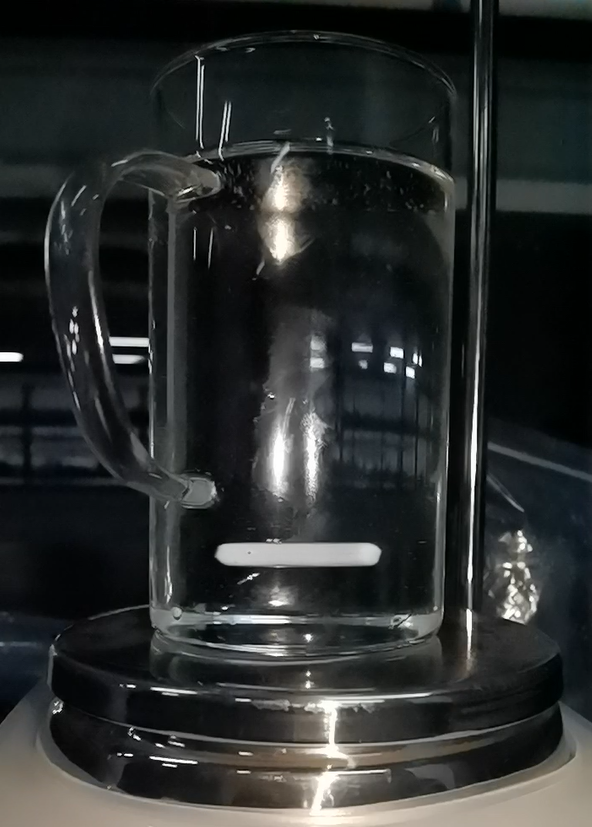
\includegraphics[height=4.5cm]{img/yushiyan.png}
			\end{figure}
		\end{itemize}
	\end{frame}
	
	\begin{frame}
		\frametitle{\fangsong{实验结果}}
		\begin{itemize}
			\item\heiti{关于假设的实验结果}\\
			\fangsong{a)观察到明显的爬杆效应。但此时在流体中放入磁子,它并没有像我们想象的那样受到爬杆效应影响而悬浮,而是可以在容器底部照常高速旋转。于是,我们可以初步否定此现象与爬杆效应的关系。}
			\begin{figure}[htbp]
				\vspace{-0.1cm}
				\centering
				\subfigure{
					\centering
					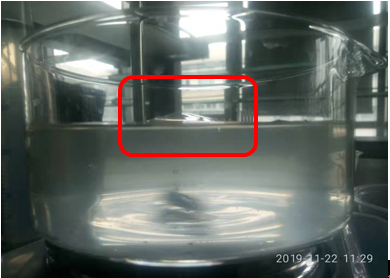
\includegraphics[height=2.5cm]{img/pagan.png}
				}
				\subfigure{
					\centering
					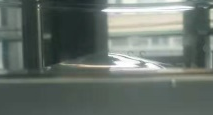
\includegraphics[height=2.5cm]{img/paganzoom.png}
				}
			\end{figure}
			\fangsong{b)在一定的转速下,磁子可以发生悬浮。虽然不是十分稳定,但可以确定是由于水的粘滞阻力小,微小的扰动就会破坏磁子的悬浮状态。这可以进一步验证此现象与爬杆效应无关。初步推断这一现象是由于搅拌器与搅拌子磁场不同步所致。}
		\end{itemize}
	\end{frame}

	\begin{frame}
	\frametitle{\fangsong{实验结果}}
	\begin{itemize}
		\item\heiti{基本量测量的结果}\\
		\fangsong{a) 实验用的甘油水溶液的密度1.302g/ml\\
			b) 实验用的甘油水溶液的粘度 \\
			c) 磁子的收尾速度 0.1318m/s
		}
	\end{itemize}
	\end{frame}

	\begin{frame}
	\frametitle{\fangsong{实验结果}}
	\begin{itemize}
		\item\heiti{定量分析}\\
		\fangsong{a) 磁子高度与搅拌器转速的关系}\\
		\qquad我们得到了磁子高度与搅拌器转速的关系图。
		\begin{figure}
			\vspace{-0.3cm}
			\centering
			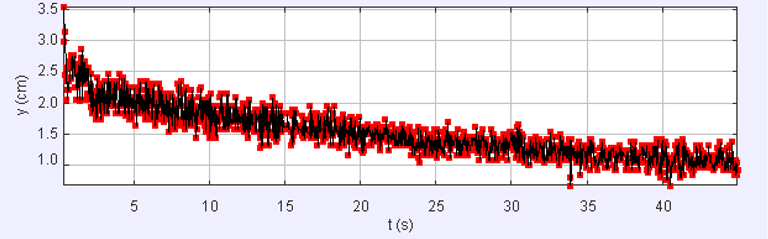
\includegraphics[height=3cm]{img/h-t.png}
		\end{figure}
		\fangsong{\qquad可以观察到起初磁子照常在结晶皿底部高速旋转,搅拌器达到一定转速时,磁子突然跳起,随后保持悬浮,并不断伴有上下振动。从图中可以看出,随着搅拌器转速不断增加,磁子悬浮的高度(上下振动的平衡位置的高度)有缓慢下降。}
	\end{itemize}
	\end{frame}

	\begin{frame}
	\frametitle{\fangsong{实验结果}}
	\begin{itemize}
		\item\heiti{b) 磁子高度变化与时间的关系}
	\end{itemize}
	\end{frame}

	\begin{frame}
	\frametitle{\fangsong{实验结果}}
	\begin{itemize}
		\item\heiti{c) 磁子旋转的角度与时间的关系}
	\end{itemize}
	\end{frame}
	
	%------------------------------------------------
	\section{\fangsong{理论部分}}
	%------------------------------------------------
	
	\section{\fangsong{数据分析}}
	\section{\fangsong{结论}}
	%------------------------------------------------
	
	\begin{frame}
		\Huge{\centerline{\fangsong{砍人大赛:街头霸王}}}
	\end{frame}
	
	%----------------------------------------------------------------------------------------
	
\end{document} 
